\documentclass{article}
\usepackage[utf8]{inputenc}
\usepackage{amsmath, amssymb}
\usepackage{bm}
\usepackage{graphicx, tikz}
\usepackage{tkz-euclide}
\usetkzobj{all}
\usetikzlibrary{calc, intersections, angles}
\addtolength{\oddsidemargin}{-2cm}
	\addtolength{\evensidemargin}{-2cm}
	\addtolength{\textwidth}{2cm}
	\addtolength{\topmargin}{-2cm}
	\addtolength{\textheight}{4cm}

\title{SMOS-HR, un modèle de dépliement le long de la trace}
\author{Eric Antérieux, François Cabot, Miguel Colom, Marina Gardella,\\ Ali Khazaal,
Yann Kerr, Jean-Michel Morel, Pablo Musé,\\ Nemesio Rodriguez, Bernard Rougé }
\date{March 2019}

\def\temp{\mathbf{\small T}}
\def\bxi{\xi}
\def\bx{\mathbf{x}}
\begin{document}

\maketitle
\section{Summary of work so far}

\subsection{Parameterizing the orbit with time}
Let $u' = (u_1', u_2', u_3')$ and $v' = (v_1', v_2', v_3')$ be two points on the arbitrary great circle $C$ through which passes the trace of a satellite orbiting the center of the earth $c=(0,0,0)$. We can take $w = \frac{u \times v'}{||u \times v'||}$ as the unit normal of the plane $P$ that intersects the sphere to produce the great circle of the orbit trace (and indeed the orbit itself). Finally, we set $u = \frac{u'}{||u'||}$ and $v = \frac{u \times w}{||u \times w||}$, and we've found an orthonormal basis of $\mathbb{R}^3$ consisting of two vectors in this plane $P$ (namely, $u$ and $v$) as well as a third unit vector $w$ that is normal to this plane.

We will derive a parametric equation for $C$ as follows by taking the parametric equation of the trace of a satellite orbiting the equator (and passing through point (R, 0, 0) at time 0),
\begin{subequations}
\label{param}
\begin{align}
    x_{eq}(t) &= R \cdot \cos(t)\\
    y_{eq}(t) &= R \cdot \sin(t)\\
    z_{eq}(t) &= 0,
\end{align}
\end{subequations}and applying a rotation:
\begin{equation} M = 
\begin{pmatrix} 
u_1 & v_1 & w_1 \\
u_2 & v_2 & w_2 \\
u_3 & v_3 & w_3
\end{pmatrix}
\end{equation}. This yields the following parametric equation for a point $p = (x,y,z)$ on the great circle $C$ as a function of time:
\begin{equation}
    p(t) = M \begin{pmatrix}
    x_{eq}(t) \\
    y_{eq}(t) \\
    z_{eq}(t)
    \end{pmatrix} = R \cdot \begin{pmatrix} u_1 \cos t + v_1 \sin t \\
    u_2 \cos t + v_2 \sin t \\
    u_3 \cos t + v_3 \sin t
\end{pmatrix}
\end{equation}

Reversing this reasoning, if we are given any two points $u'$ and $v'$ on a great circle of radius $R$, we can construct two orthonomal points $R \cdot (u_1, u_2, u_3)$ and $R \cdot (v_1, v_2, v_3)$ and apply the inverse rotation $M^{-1} = M^T$ to these two points to arrive back at Eqs. ~\eqref{param}.

(Knowing the period $T$ of the orbit, we can sample $t$ at appropriate values $2\pi\frac{t_i}{T}$ to ensure our samples and sample interval reflect the satellite's speed.) 

\subsection{Coordinate system around satellite}

Let $\mathbf{r}(t)$ be the satellite's position with respect to an inertial frame. Its direction of motion is $\mathbf{y}(t) = \mathbf{r}(t)/||\mathbf{r}(t)||$, the negative of its angular momentum vector $\mathbf{x}(t) = -(\mathbf{r}(t) \times \mathbf{r}'(t))/||\mathbf{r}(t) \times \mathbf{r}'(t)||$, and $\mathbf{z}(t) = \mathbf{y}(t) \times \mathbf{x}(t)$ is the unit vector that completes the right-handed coordinate system. Here at any fixed time $t$ the $y$ axis defined by the $\mathbf{y}(t)$ points in the direction of motion, and we have let $x$ axis point ``down" (ie, along a line parallel to the line between the center of Earth and the South Pole as the satellite orbits counterclockwise around the equator), and positive $z$ axis point directly away from the center of Earth (and the subsatellite point) from the satellite's position.

Given a point $(x,y,z)$ in Cartesian coordinates, we use the following definition of spherical coordinates (the ``physics" rather than the ``math" definition). A point in 3D space, relative to the origin, is given by the triple ($\rho, \theta, \phi)$, which are defined as the distance of the point to the origin, the colatitude (ie, the angle $\in [0, \pi ]$ taken from the positive $z$-axis), and the azimuth (ie, the angle from the positive $x$-axis, $\in [0,2\pi])$ . Values of $\phi \in (0, \pi/2) \cup (3\pi/2, 2\pi)$ point away from Earth.

 We can then define
\begin{subequations}
\begin{align}
\xi &= \frac{x}{\rho} = \sin \theta \cdot \cos \phi \textnormal{, and } \label{xi1}\\ 
\eta &= \frac{y}{\rho} = \sin \theta \cdot \sin \phi \label{eta1}.
\end{align}
\end{subequations}

We define $\bm{\xi}(t) = (\xi(t), \eta(t)).$ This point lies in the unit disk as $\xi^2 + \eta^2 = \sin^2 \theta (\cos^2 \phi + \sin^2 \phi) = \sin^2 \theta \leq 1.$ In Cartesian coordinates, this relation becomes the following: $0 \leq \frac{x^2+y^2}{x^2+y^2+z^2} \leq 1$.

Knowing the azimuth $\theta$, or equivalently (in Figures 1-2) $u$, the look angle from the satellite to the point of observation relative to the negative $z$ axis, one can trace out a ``cone of confusion" which forms a circle of confusion if one knows $\rho$ as well. For appropriate $\rho$, if $u \leq 64.6$ degrees, this circle of confusion will be a locus of points on Earth's surface (see Figure 1). The azimuth value specifies how far around this circle of confusion we must travel to identify the target point being observed.

Knowing $\eta$ and $\xi$, we can specify a ray on this cone. The value $\sin \theta = \sin (\pi - \theta)$ is the ratio between the radius of the circle of confusion and $\rho$, its distance from the satellite. This is the scale factor. Since $\phi$ gives us the angular distance around the circle we've traveled from the positive $x$-axis (ie, starting at the point nearest the South Pole when the trace of the satellite is the Equator, and moving counter-clockwise), $(\cos \phi, \sin \phi)$ gives us the coordinates of the observed point on the circle if it were scaled to the unit circle. Thus, we have a point on the unit circle, and we know how much this unit circle gets scaled as $\rho$ increases, we have specified a ray. 

Where does this ray intersect with Earth? Given a satellite at height $h$ and given that Earth's radius is $R$, we can compute both the radius of this circle $r$ and $\phi$ by considering the triangle CTR-OBS-SAT, where CTR is the center of Earth, OBS is a point on the circle, and SAT is the satellite. The segment from CTR to OBS has length $R$, the segment from OBS to SAT $\rho$, and the segment from SAT to CTR has length $R+h$. The angle OBS-SAT-CTR is $\pi - \theta$. Let $\alpha$ be the angle SAT-CTR-OBS. Thus from the law of sines and the fact that $\sin (\pi - \theta) = \sin \theta$, we obtain the following relation:
\begin{equation}
    \sin \frac{\theta}{R} = \sin \frac{\alpha}{\rho} \label{lawofsines}.
\end{equation} 
From the law of cosines, we can solve for $\rho$: 
\begin{equation}
    R^2 = \rho^2 + (R+h)^2 + 2 \rho (R+h)\cos \theta \label{lawofcosines}.
\end{equation}

Having obtained $\rho$ and knowing $\theta$, we can find the radius of the circle using $r = \rho \sin \theta$.

Thus, knowing $\bm{\xi}$ as well as $R$ and $h$ (and, it will turn out, the hemisphere of observation), we can uniquely identify the point where this ray intersects Earth, for any fixed location of the satellite. If the satellite is at $(x,y,z) = (0,0,0)$, we can easily obtain the $(\rho,\theta,\ohi)$ coordinates of this point, using the following algorithm:

Step 1. Compute $\theta = \pi - \sin^{-1}\big(\sqrt{\xi^2 + \eta^2}\big)$, where we assume the range of $\sin^{-1}: [-1,1] \rightarrow \mathbb{R}$ is $[0, \pi]$. We don't have to worry about the ``negative square root" because this corresponds to pointing away from Earth.

Step 2. Compute $\phi = \tan^{-1}\big(\frac{\eta}{\xi}\big)$. When the range of $\tan^{-1}: \mathbb{R} \rightarrow \mathbb{R}$ is defined as $[-\pi/2, \pi/2]$, this gives a point in the Southern Hemisphere. Add $\pi$ to the angle to consider a point in the Northern Hemisphere.

Step 3. Using Eq.~\eqref{lawofcosines}, we can determine $\rho$.


% As the satellite traces its circular orbit, $\bm{\xi}(t)$ traces out an ellipse within the unit disk.

%What do the Cartesian coordinates associated with this spherical coordinate system correspond to? We define the $x$ axis as the yaw axis, where $x$ increases as one moves directly ``down" from the satellite toward the center of Earth; the $y$ axis as the pitch axis, where $y$ increases as one moves to the ``left" of the satellite if one faces in the direction of its motion (which we have made counterclockwise along the equator in the visualizations when the ``north pole" is above the equator, so that along the trace of the satellite's orbit, pitch increases due north); and the $z$ axis as the roll, which corresponds to ``forward" motion along the tangent line to the satellite's motion.

%Thus, the spherical coordinate $\theta$ is 0 when the satellite is looking straight ahead, $\pi/2$ when looking down, and $\pi$ when looking backward, and the spherical coordinate $\phi$ is 0 when the satellite is looking down, $\pi/2$ when looking left, $\pi$ when looking up, and $3\pi/2$ when looking right. If the satellite is at altitude $h$, the subsatellite point is at $(\rho, \theta, \phi) = (h,\pi/2,0)$, and a point $m$ units of circumference directly ``ahead" of the satellite on its trace will have coordinates  $(d, \theta, 0)$ that can be identified by applying the law of sines and the law of cosines to the triangle consisting of the satellite SAT, the center of Earth CTR, and the point along the trace being observed OBS, where the angle $u$ is formed between OBS, SAT, and CTR and $\gamma$ is the angle between SAT, CTR, and OBS and (when measured in radians) is just $\frac{m}{R}$:


%What do the Cartesian coordinates associated with this spherical coordinate system correspond to? We define the $x$ axis as the yaw axis, where $x$ increases as one moves directly ``down" from the satellite toward the center of Earth; the $y$ axis as the pitch axis, where $y$ increases as one moves to the ``left" of the satellite if one faces in the direction of its motion (which we have made counterclockwise along the equator in the visualizations when the ``north pole" is above the equator, so that along the trace of the satellite's orbit, pitch increases due north); and the $z$ axis as the roll, which corresponds to ``forward" motion along the tangent line to the satellite's motion.

%Thus, the spherical coordinate $\theta$ is 0 when the satellite is looking straight ahead, $\pi/2$ when looking down, and $\pi$ when looking backward, and the spherical coordinate $\phi$ is 0 when the satellite is looking down, $\pi/2$ when looking left, $\pi$ when looking up, and $3\pi/2$ when looking right. If the satellite is at altitude $h$, the subsatellite point is at $(\rho, \theta, \phi) = (h,\pi/2,0)$, and a point $m$ units of circumference directly ``ahead" of the satellite on its trace will have coordinates  $(d, \theta, 0)$ that can be identified by applying the law of sines and the law of cosines to the triangle consisting of the satellite SAT, the center of Earth CTR, and the point along the trace being observed OBS, where the angle $u$ is formed between OBS, SAT, and CTR and $\gamma$ is the angle between SAT, CTR, and OBS and (when measured in radians) is just $\frac{m}{R}$:

%\begin{align}
%    R^2 &= (R+h)^2 + d^2 -2(R+h)d\cos u\\
%    \frac{\sin \gamma}{d} &= \frac{\sin u}{R}.
%\end{align} See Figure 2.

\subsection{Calculating planar coordinates $x, y,$ and $ \theta$ on the unit disk}
Caution: In this section, $x$, $y$, and $\theta$ will take on second meanings. They will continue to refer to the $x$-, $y$-, and colatitude coordinates in $\mathbb{R}^3$, respectively. But they will also refer to the following new coordinates under a mapping from the unit disk to the plane. If we perform a rotation of the sphere such that the great circle that is the satellite's orbital trace is the equator, $x$ is the ``vertical arc length" from the subsatellite point on the equator to the observed point (ie, $R$ times the magnitude of the latitude---in radians---of the observed point) and $y$ the ``horizontal arc length" (ie, $R$ times the angular distance between the subsatellite point and the observed point's spherical-triangular projection onto the equator). Additionally, $\theta$ is the look angle between a point on the ground and the satellite in orbit. We have rechristened this angle $\gamma$ in an attempt to lessen our confusion.

Moreover, it’s important to make a clear distinction between $\bm{\xi}$ and $\xi$
as for instance $y$
visits a particular $\xi$
twice per orbit, it visits a unique pair $(\xi, \eta)$ at most once per orbit. Reflecting on its definition in rectanglular coordinates, it's immediately clear that $\bm{\xi}$ does not depend on $R$.

First, we assume that the satellite is orbiting so that its trace traverses the ``equator" of the sphere, starting at time 0 at point $(x_G,y_G,z_G) = (R,0,0)$ in a standard geocentric Cartesian coordinate system. (This rotation can be achieved with $M^{-1}$.) Given that we're on this sphere of radius $R$ we need use only two coordinates to define a point on the sphere: $x_{angular}$, the latitude ($\frac{\pi}{2} - \theta)$, where $\theta$ is the colatitude in our definition of geocentric spherical coordinates), and $y_{angular}$, the azimuth (the $\phi$ parameter in our definition of geocentric spherical coordinates). Equivalently, we can define $x$ and $y$ in terms of arc length instead of angle in radians. This can be done by setting $x = Rx_{angular}$ and $y = Ry_{angular}$.  The trace of the satellite can then be parameterized by time, for instance as (0, $y(t)$) where $y(0) = 0$, and $y(T) = 2R\pi$ where $T$ is the period of orbit.

We wish to characterize the point of observation, OBS, in terms of these coordinates. It depends on both the position of the satellite\footnote{With respect to OBS: our satellite remains at the origin of the coordinate system throughout the orbit, but the point OBS ``moves" with respect to this system.} and the orientation $\bm{\xi}$ of the satellite. 

Consider the right spherical triangle whose hypotenuse is the arc between the point OBS and the subsatellite point SSP, and whose third point is TR, the projection of OBS onto the trace of the orbit. The angular distance between OBS and TR is $x' = x/R$ and the angular distance between TR and SSP is $y' = y/R$. From Napier's rules for spherical trigonometry, we get the following equation to compute $\gamma$, the angular distance between OBS and SSP:
\begin{equation}
    \cos \gamma = \cos \big(\frac{x}{R}\big)\cos \big(\frac{y}{R}\big) \label{napier}.
\end{equation}

%We can further use the fact that $\angle$OBS-TR-SSP is right to get that $0 = \tan \frac{x}{R} \cot \frac{y}{R}$

Given a point OBS = $(x,y)$ on Earth, we will compute its spherical coordinates $(\rho, \theta, \phi)$ with respect to the satellite SAT. Consider the triangle between CTR, the center of the earth, OBS, and the actual position of the satellite in space, SAT (Figure 2). SAT is of distance $R+h$ from the CTR and OBS and the subsatellite point SSP are both of distance $R$. We can use the law of cosines since we have the angular distance between the satellite SAT and the observer OBS (which happens to be the same as the angular distance between the observer and the subsatellite point on the trace), namely $\gamma$. Hence the Cartesian distance $d$ between the point being observed on the earth and the satellite is as follows:
\begin{align*}
    d^2 &= R^2 + (R+h)^2 -2R(R+h)\cos\gamma\\
    &= R^2 + (R+h)^2 -2R(R+h) \cos \big(\frac{x}{R}\big)\cos \big(\frac{y}{R}\big),
\end{align*} where the second line applies Eq.~\eqref{napier}, so that 
\begin{equation}    
    d = (R+h) \cdot \sqrt{1 + \bigg(\frac{R}{R+h}\bigg)^2 - 2 \frac{R}{R+h}\cos \big(\frac{x}{R}\big)\cos \big(\frac{y}{R}\big)}
\end{equation}
We can then use the law of sines to compute $v$, the look angle from OBS to SAT:
\begin{equation*}
    \frac{\sin (v+\frac{\pi}{2})}{R+h} = \frac{\sin \gamma}{d},
\end{equation*}
and so 
\begin{equation}
v = \cos^{-1}\bigg(\frac{R+h}{d} \sin \gamma\bigg)
\end{equation}
This angle $z$ is the $\frac{\pi}{2}$-complement to the look angle $\theta$, which we can therefore write as follows:
\begin{align}
    \theta(\xi, \eta) &= \cos^{-1}\bigg(\frac{R+h}{d} \sin \gamma\bigg) \\
    & = \cos^{-1}\bigg(\frac{\sin(x) \cos(y(\bm{\xi}) - y)}{\sqrt{1 + \bigg(\frac{R}{R+h}\bigg)^2 - 2 \frac{R}{R+h}\big(\sin(x) \cos(y(\bm{\xi}) - y)\big)}}
\bigg)
\end{align}


\begin{figure}
\begin{tikzpicture}[vert/.style args={of #1 at #2}{insert path={%
#2 -- (intersection cs:first
  line={#1}, second line={#2--($#2+(0,10)$)}) }},
vert outwards/.style args={from #1 by #2 on line to #3}{insert path={
#1 -- ($#1!#2!90:#3$)
}}]


\path [rotate=-15]
  (0,0)   coordinate (HOR) 
  (0,-3) coordinate (CTR) 
  (5,0)  coordinate (SAT);

  
\path [name path=first]  (HOR) -- (SAT);
\path [name path=second] (HOR) -- (CTR);
\path [name path=third] (CTR) -- (SAT);

\draw let \p1=(HOR), \p2=(CTR), \n1={veclen(\x2-\x1,\y2-\y1)} in (CTR) circle [radius=\n1];
\draw (HOR) -- (SAT);
\draw (CTR) -- (HOR);
\draw (CTR) -- (SAT);

\tkzMarkRightAngle[size=.4](CTR,HOR,SAT);
\foreach \p/\a in {HOR/above,CTR/below,SAT/right}
  \node [inner sep=1pt, circle, fill, label=\a:\p] at (\p) {};

\tkzInterLC(CTR,SAT)(CTR,HOR) \tkzGetSecondPoint{SSP}
\tkzDrawPoints(SSP);
\tkzLabelPoints(SSP);

\draw[name path=line1,dashed,vert outwards={from {($(CTR)!0.9999!(SAT)$)} by 1cm on line to {(SAT)}}];
\draw[name path=line2,dashed,vert outwards={from {($(CTR)!0.9998!(SAT)$)} by -1cm on line to {(SAT)}}];
%\draw [name intersections={of=circle and axis, by=x}] (x) circle (1pt);

\tkzLabelSegment[left=3pt](HOR,CTR){$R$};
\tkzLabelSegment[below=3pt](CTR,SSP){$R$};
\tkzLabelSegment[below=3pt](SSP,SAT){$h$};
\tkzLabelSegment[pos=0.9](HOR,SAT){$\gamma$};
\tkzLabelAngle[pos = -0.8](HOR,SAT,CTR){$u$};
\tkzLabelAngle[pos=0.85](HOR,CTR,SAT){$\gamma$};
\pic [draw=black, angle radius=1.2cm] {angle = HOR--SAT--SSP};
\pic [draw=black,-,angle radius=0.5cm] {angle = SAT--CTR--HOR};

\tkzTangent[from with R = SAT](CTR,5.83095cm)  \tkzGetPoints{R}{I} %SQRT(25+9)
\tkzMarkRightAngle[size=.4](CTR,SAT,I);



\end{tikzpicture}
\caption{A cross-section of Earth, the satellite's position labeled SAT, the subsatellite point SSP, the center of the Earth CTR, and the horizon HOR.The dashed line represents the tangent to the satellite's instantaneous path. Here the angular distance between the horizon and the subsatellite point $\gamma$ is equal to $\pi/2 - u$, where $u$ is the angular radius of Earth. Here $\gamma = \cos^{-1} \frac{R}{R+h} \approx 0.445$ radians, thus the distance between the satellite and the horizon point is $(R+h)\sin \theta \approx 3037$ km when $R=6371$ km and $h=687$ km. Since the satellite can see in this direction between the subsatellite point and the horizon, its field of view is roughly $u = \frac{\pi}{2} - 0.445$ radians or about 64.6 degrees.}
\end{figure}


\begin{figure}
\begin{tikzpicture}[vert/.style args={of #1 at #2}{insert path={%
#2 -- (intersection cs:first
  line={#1}, second line={#2--($#2+(0,10)$)}) }},
vert outwards/.style args={from #1 by #2 on line to #3}{insert path={
#1 -- ($#1!#2!90:#3$)
}}]


\path [rotate=0]
  (0,0)   coordinate (TOP) 
  (0,-4) coordinate (CTR)
  (7,-1)  coordinate (SAT)
  (7,-2.5) coordinate (RIGHT);
  
\tkzInterLC(TOP,RIGHT)(CTR,TOP) \tkzGetSecondPoint{OBS}

\tkzInterLC(CTR,SAT)(CTR,OBS) \tkzGetSecondPoint{SSP}
\tkzDrawPoints(SSP);
\tkzLabelPoints(SSP){SSP};

\tkzTangent[from with R = OBS](CTR,4cm)  \tkzGetPoints{R}{I}
\tkzDrawLine[dashed,add=-3 and -3](R,I);

\draw let \p1=(TOP), \p2=(CTR), \n1={veclen(\x2-\x1,\y2-\y1)} in (CTR) circle [radius=\n1];
  
\path [name path=first]  (OBS) -- (SAT);
\path [name path=second] (OBS) -- (CTR);
\path [name path=third] (CTR) -- (SAT);

\draw (OBS) -- (SAT);
\draw (CTR) -- (OBS);
\draw (CTR) -- (SAT);
\draw (SSP) -- (SAT);

\foreach \p/\a in {OBS/above,CTR/below,SAT/right}
  \node [inner sep=1pt, circle, fill, label=\a:\p] at (\p) {};


\draw[name path=line1,dashed,vert outwards={from {($(SSP)!0.9999!(SAT)$)} by 1cm on line to {(SAT)}}];
\draw[name path=line2,dashed,vert outwards={from {($(CTR)!0.9998!(SAT)$)} by -1cm on line to {(SAT)}}];
\draw[name path=line3,dashed,vert outwards={from {($(R)!0.5!(I)$)} by 1cm on line to {(I)}}];
%\draw[name path=line3,dashed,vert outwards={from {(OBS)} by -1cm on line to {(CTR)}}];
%\draw [name intersections={of=circle and axis, by=x}] (x) circle (1pt);

\tkzMarkRightAngle[size=.4](CTR,OBS,R);

\tkzLabelSegment[left=3pt](OBS,CTR){$R$};
\tkzLabelSegment[below=3pt](CTR,SSP){$R$};
\tkzLabelSegment[below=3pt](SSP,SAT){$h$};
\tkzLabelSegment[pos=0.4](OBS,SAT){$d$};
\tkzLabelAngle[pos = -0.8](OBS,SAT,CTR){$u$};
\tkzLabelAngle[pos=0.6](OBS,CTR,SAT){$\gamma$};
\tkzLabelAngle[pos=0.4](I,OBS,SAT){$v$};
\pic [draw=black, angle radius=1.2cm] {angle = OBS--SAT--SSP};
\pic [draw=black,-,angle radius=1cm] {angle = SAT--CTR--OBS};
\pic [draw=black, angle radius=0.65cm] {angle = I--OBS--SAT};

\tkzTangent[from with R = SAT](CTR,7.61577cm)  \tkzGetPoints{R}{I} %SQRT(49+9)
\tkzMarkRightAngle[size=.4](CTR,SAT,I);


\end{tikzpicture}
\caption{A cross-section of Earth, the satellite's position labeled SAT, the subsatellite point SSP, the center of the Earth CTR, and the point being obsered, OBS. The dashed lines represent the tangent to the satellite's instantaneous path and a cross-section of the tangent plane to the spherical earth through the point OBS. The angular distance between the horizon and the subsatellite point is given by $\gamma$ and is now less than the observed point's spherical coordinate $\theta$.}
\end{figure}
\iffalse
\subsection{Scratch}

From the first (ie, the Cartesian, not spherical) relation in Eq.~\eqref{xi1}-~\eqref{eta1} and from the parameterized orbits Eq.~\eqref{x1}-~\eqref{y1}, it follows from this parameterization of the orbit that we can parameterize $\xi$ and $\eta$:
\begin{subequations}
\begin{align*}
\xi(t) &= \frac{x(t)}{\rho} = \frac{1}{R} \cdot (x_1 \cos t + x_2 \sin t \label{x1}) \textnormal{, and }\\ 
\eta(t) &= \frac{y(t)}{\rho} = \frac{1}{R} \cdot( y_1 \cos t + y_2 \sin t).
\end{align*}
\end{subequations}

With respect to the ``physics" spherical coordinate system, we can write
\begin{align}
\xi(\theta, \phi) &= \sin \theta \cdot \cos \phi \\
\eta(\theta, \phi) &= \sin \theta \cdot \sin \phi.  
\end{align}
 Changing coordinates so that $x = \frac{\pi}{2} - \theta$ and $y = \phi$ this becomes
 \begin{align}
\xi(x, y) &= \cos x \cdot \cos y \label{one}\\
\eta(x, y) &= \cos  x \cdot \sin y \label{two}.  
\end{align}

Solving Eq. \eqref{one} for $\cos x$ and plugging the result into Eq. \eqref{two}, we get that 
\begin{equation}
    y(\bm{\xi}) = y(\xi, \eta) = \tan^{-1}\bigg(\frac{\eta}{\xi}\bigg).
\end{equation}

By recognizing that $\xi^2+\eta^2 = \cos^2 x(\sin^2 y + \cos^2 y)$, we get that 
\begin{equation}
    x(\bm{\xi}) = x(\xi, \eta) = \cos^{-1}\big(\pm \sqrt{\xi^2 + \eta^2}\big) = \bigg\{\cos^{-1}\big(\sqrt{\xi^2 + \eta^2}\big), \cos^{-1}\big(\sqrt{\xi^2 + \eta^2}\big) + \frac{\pi}{2}\bigg\}.
\end{equation}
TODO investigate, specify as a function

Finally, we are interested in $\theta(\bm{\xi})$ where $\theta$ is the angle between some point $P$ and the satellite's position at a given time.
\fi



  \section{Analyse numérique}
  On  doit  faire deux simulateurs. Pour les deux, il faut commencer par  préciser  des versions simplifiées des  formules et  de la géométrie,  pour  arriver au plus vite à simuler numériquement une acquisition et une restitution de la température de brillance.
  \paragraph{Spécifications des formules}
  \begin{itemize}
      \item Formules de $x(\xi), y(\xi), \theta(\xi)$ où on suppose que la terre est parfaitement sphérique de rayon $R$ et que le satellite sera placé sur un grand cercle d'altitude $h$
      \item  coordonnées discrètes des  points $x(\eta_i, 0)$ où $\eta$ est la seconde coordonnée de $\xi$ et est  un cosinus directeur et les $\eta_i$ sont échantillonnées régulièrement. 
       \item Formules des $\phi_i(x)$, B-splines cubiques\newline \url{https://en.wikipedia.org/wiki/B-spline}, \url{https://fr.wikipedia.org/wiki/B-spline}\newline (par exemple) dont les  points de contrôle sont un ensemble irrégulier de points,  en l'occurrence les $\eta_i$
       \item Pour  les $f_i$ on peut prendre $f_i(\theta)=\theta^i$, $i=0, \cdots m$ and $m=4$
       \item Dans ce modèle légèrement simplifié on commencera par prendre $r_{kl}\equiv 1$, $F_k(\xi)=(1-|\xi|^2)$, $u_{kl}=(k,l)\in [-L,  L]\cap\mathbb{Z}$ sont des entiers.
       \end{itemize}
       
       \paragraph{Simulation des visibilités} Le premier but est de simuler les  données observées telles que données par \eqref{echantillonageFourier2bis}. Pour cela  on se  donne une  image  rectangulaire RGB du type  planisphère satellitaire comme celle indiquée ci-dessous et  on acquiert donc une suite de $N$ clichés circulaires de cette image de gauche à droite, de diamètre inférieur à la hauteur  l'image. On acquiert  $N$ clichés et on traite  le planisphère comme une image  périodique de  période $N$.
        Avec cela on  peut calculer numériquement les coefficients du système \eqref{echantillonageFourier4} pour  chaque  $k,l$. Donc:  
        
\begin{itemize}
    \item Input: $u$ le planisphère de  dimensions $M\times N$, $L<< \frac N2$,  $m\leq 2$ (premiers tests avec $m=0$)
    \item Output:  série de $N$ clichés, chacun est une matrice de visibilités $V_{kl}^y$, $y=1, \cdots N$, obtenu en centrant le cercle d'acquisition aux $N$ positions  $(y, \frac N2)$, $y=1,  \cdots N$.
\end{itemize}


  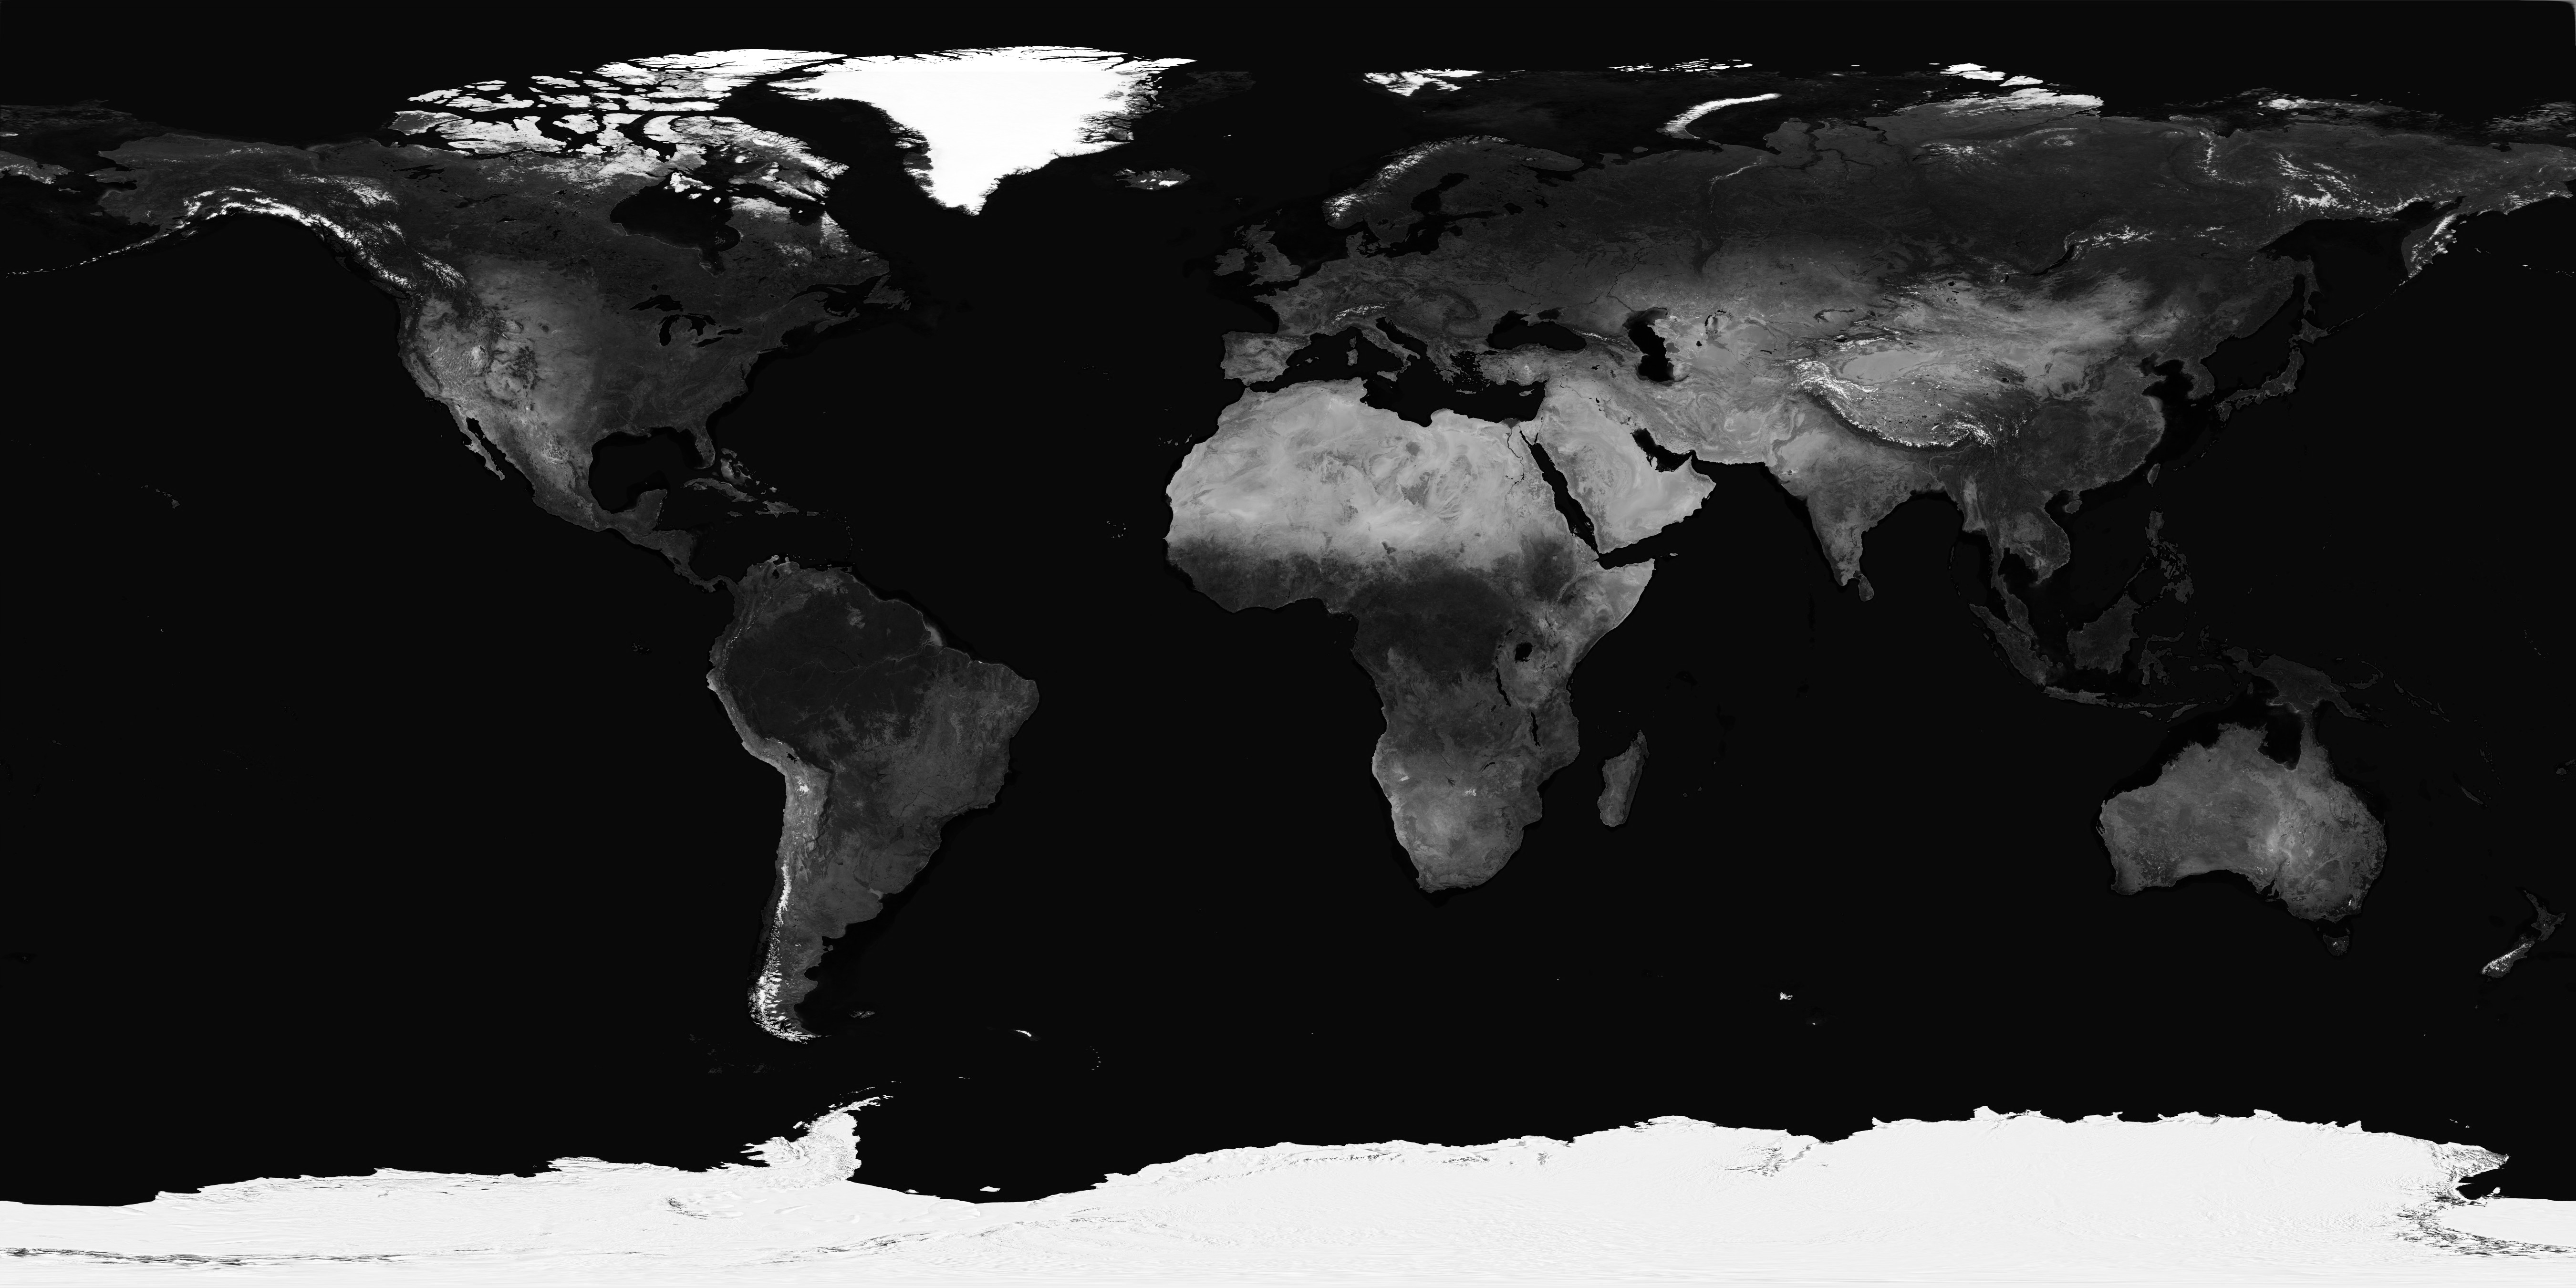
\includegraphics[width=0.8\textwidth]{PlanisphereSatellite.png}
  
       \paragraph{Simulation de l'inversion}
    \begin{itemize}
    \item Input:  série de $N$ clichés, chacun est une matrice de visibilités $V_{kl}^y$, $y=1, \cdots N$
    \item Output: paramètres $\alpha(x,y)$ de la température de brillance
        \item  On commence par appliquer la transformée de Fourier partielle en $y$ aux coefficients $y\to V_{kl}^y$ pour obtenir les matrices $\tilde V_{kl}(\omega),$ $\omega = 1,\cdots N$.
         Ensuite on doit faire une pseudo inversion de du système d'équations  
         
\item  Ces $(2L+1)^2$ équations  sont résolues indépendamment pour chaque $\omega$! Une fois que c'est fait, on  applique la transformée partielle inverse à $\tilde \alpha(x,\omega)$ définie par \eqref{coefficientsplinedealpha} pour déduire la fonction $\alpha(x,y).$

\end{itemize}
  
  
  \section{Glossaire}
  tilt/pitch, yaw/pan,  roll
  Altitude du satellite: 687 km
  Rayon de la terre: 6371
  Distance à l'horizon: 3037
  Angle de vue du ciel : 25.5$^\circ$
  
 \end{document}

